\subsection{Input, Output, State}
    %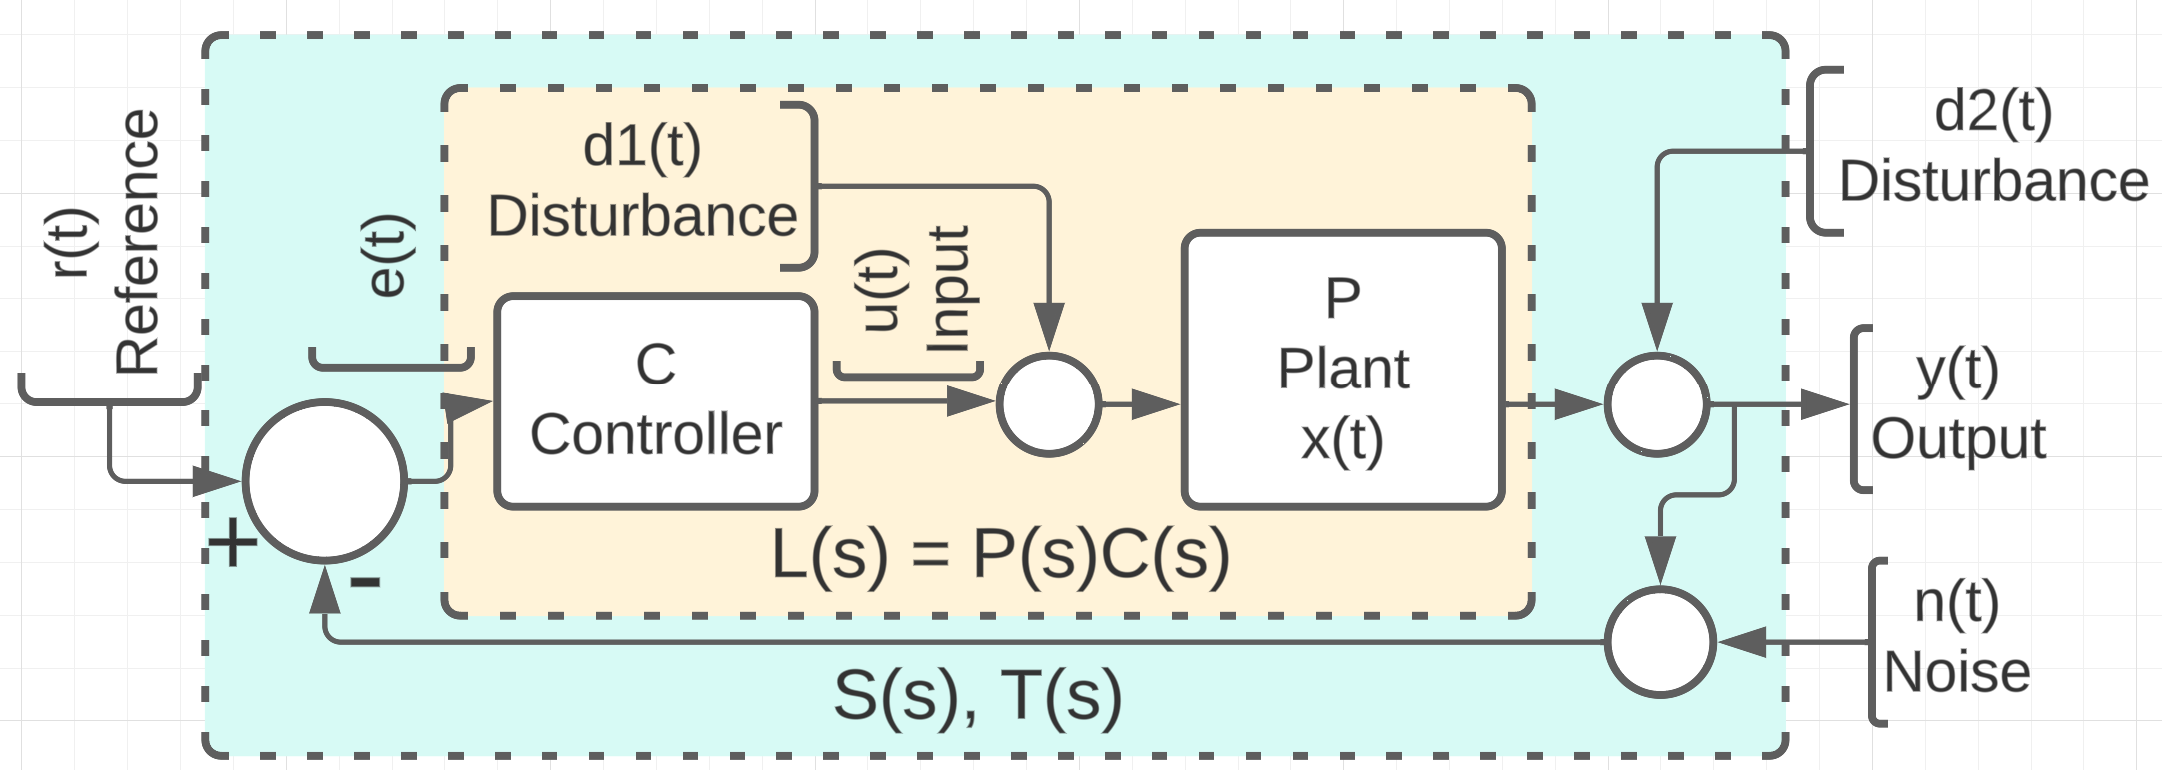
\includegraphics[width = \linewidth]{src/images/basic_block_chart.png}
    \begin{itemize}
        \item \textbf{(Control) Input u(t)} (gas pedal)
        \begin{itemize}
            \item endogenous: manipulation by designer
            \item exogenous: generated by environment (e.g. Weather)
        \end{itemize}
        \item \textbf{Output / Measurement y(t)} (speed)
        \begin{itemize}
            \item measured outputs: Quantities that we can measure
            \item performance outputs: unmeasurable but controllable (e.g. average fuel consumption)
        \end{itemize}
        \item \textbf{state x(t)}: "memory", summary of all past inputs (fuel)
        \item parameter: quantities that do not change over time (colour)
\end{itemize}